\documentclass[oneside]{hpman}

\usepackage{tikz}

\title{HPCAP}
\subtitle{Developer guide}
\author{Guillermo Juli\'an Moreno}
\authormail{guillermo.julian@estudiante.uam.es}
\date{\today}

\settocdepth{subsubsection}
\makeindex[intoc]

\begin{document}

\begin{abstract}
The HPCAP Developer Guide has all the necessary information for developers and maintainers of the HPCAP driver and client applications. It includes a description of inner workings of the driver, how the code is structured and the auxiliar tools created to support the development and the driver.
\end{abstract}
\maketitle

\tableofcontents
\newpage

\chapter{Introduction, basic information and practices}

The HPCAP driver is a modification of the Intel IXGBE driver that allows capture of traffic at high rates. This section acts as a basic introduction to the driver code and development practices.

This document, along with the auto-generated code manuals, the user guide and V\'ictor Moreno's master's thesis \cite{MorenoTFM2012}, conform the documentation of the HPCAP driver.

\section{Folder structure}
\label{sec:dirs}

The HPCAP driver code tree is structured as follows:

\begin{itemize}
\itemdescit{Doxyfile} The instruction file that generates Doxygen documentation. See \fref{sec:doxygen} for details.
\itemdescit{Makefile} The file with instructions for the build system. See \fref{sec:build}.
\itemdescit{Makefile-driver-vars.mk} Specific Makefile code to set the driver build configuration.
\itemdescit{doc} The folder that contains the documentation for the HPCAP driver. The folders \fileobj{doc/latex}, \fileobj{doc/html} and \fileobj{doc/man} contain the autogenerated Doxygen documentation in each respective format.
\itemdescit{driver} Contains the source files for the driver. This folder contains three subdirectories:
\begin{itemize}
\itemdescit{hpcap\_ixgbe-4.1.2} IXGBE driver files.
\itemdescit{hpcap\_ixgbevf-2.14.2} IXGBE driver files - virtual mod.
\itemdescit{common} Common files for both drivers (i.e., HPCAP-related files)
\end{itemize}
\itemdescit{include} C header files.
\itemdescit{install\_hpcap.bash} Driver install script.
\itemdescit{params.cfg} Driver configuration file.
\itemdescit{samples} Sample applications. See \fref{sec:samples}.
\itemdescit{scripts} Helper scripts.
\itemdescit{srclib} Library source codes. See \fref{sec:libs}.
\itemdescit{bin} Binary output folder. Samples binaries and modules will be stored here.
\itemdescit{obj} Output folder for the compilation intermediate products.
\end{itemize}

\section{Version control}

The version control system used by HPCAP is SVN. The branching strategy is discussed below. To aid maintenance and development, the developer should follow \href{http://chris.beams.io/posts/git-commit/}{usual recommendations regarding commit messages}. Basically, ensure that commit messages describe what was done and why, not how (we already have the diff to see how it was done).

It's also helpful to include the ``category'' of the commit in the subject line, such as ``hpcap: Fix reset of listener's buffer size'' or ``lib: Refactor listener operations in a common function''. As HPCAP has several different parts, this helps to understand what has been changed without too much explaining (e.g., it's not the same to change listener code in the hpcap driver than in the library, and the prefix ``hpcap:'' or ``lib:'' takes care of that) and also helps when reading the commit log.

Commits should also be atomic, that is, one commit should reflect one change in the codebase. This helps a lot when reverting specific features or when searching where was a bug introduced.

\section{Version numbers}
\label{sec:versioning}

From version 4.2.0 onwards, HPCAP follows the \href{http://semver.org/}{semver} semantic versioning scheme. This means that version numbers are of the form \textit{MAJOR.MINOR.PATCH}.

New versions should increment one of the tree numbers:

\begin{itemize}
\item \textit{MAJOR} version when the API changes in incompatible ways.
\item \textit{MINOR} version when new functionality is added in backwards-compatible manner.
\item \textit{PATCH} version when there are new backwards-compatible bugfixes.
\end{itemize}

\section{Code formatting}

The HPCAP code is formatted using the \href{https://www.kernel.org/doc/Documentation/CodingStyle}{Linux coding style guide}, using tabs for indentation. To make formatting easier, the file \fileobj{.astylerc} contains the options to format the code with the \href{http://astyle.sourceforge.net/astyle.html}{astyle} tool. You can format manually the code executing \texttt{astyle --options=.astylerc -R "./*.c" "./*.h"}, or you can integrate this options file with editors that support automatic formatting, such as Sublime Text's \href{https://github.com/timonwong/SublimeAStyleFormatter}{AStyleFormatter} or Vim's \href{https://github.com/Chiel92/vim-autoformat}{Autoformat}.

\section{Doxygen documentation}
\label{sec:doxygen}

This document contains general documentation regarding the driver and related software. For more specific documentation about the code, \href{http://www.stack.nl/~dimitri/doxygen/}{Doxygen}-style comments are used. The advantage of this comment style is that developer-friendly documentation can be generated automatically. The file \textit{Doxyfile} controls this documentation output. Currently, HTML, LaTeX and \index{man}Man versions of the documentation are generated. To explore the generated manpages, you should change your \texttt{MANPATH} variable running the command \texttt{export MANPATH=\$MANPATH:hpcap-path/doc/man}. Alternatively, you can run \texttt{sudo make install} to install everything to your system, including the manpages.

\chapter{Build and installation system}
\label{sec:build}

The build system used for HPCAP is, as always, GNU Make. Apart from the traditional \texttt{all} target that builds everything, there are three other targets:

\begin{itemize}
\item \texttt{samples}. These are applications built for this driver, with the purpose of either aiding development and debugging or as simple utilities, such as the hugepage mapper or the \textit{hpcapdd} dumper. The samples are described in \fref{sec:samples}.
\item \texttt{libs}. To allow using the HPCAP driver from userspace applications, two libraries act as layers between them and the driver. These are described in \fref{sec:libs}.
\item \texttt{drivers}. The \textit{hpcap} and \textit{hpcapvf} drivers, no need to say what are they. The targets \texttt{drivers-release} and \texttt{drivers-debug} may be used to create debug or release versions of the drivers.
\item \texttt{install} and \texttt{uninstall}. These targets respectively install and uninstall the HPCAP from the driver. The installation procedure is explained in \fref{sec:install}.
\end{itemize}

To build all the targets, there is a Makefile placed in the root of the code tree. It builds the samples, libraries and drivers detecting automatically the dependencies. In order for it to work, it needs a strict folder structure as described in \fref{sec:dirs}.

The restrictions are the following:

\begin{enumerate}
\item Each sample should be in its own directory inside of \textit{samples}. If there are multiple samples in one directory (that is, more than one file with a \texttt{main} function) compilation will fail.
\item Library header files should be kept in the \textit{include} directory.
\item Library code files should be kept in the \textit{srclib/libname} directory.
\item Kernel drivers must be placed in the \textit{driver} directory. Each driver should be named \textit{hpcap\_ixgbe[extra]-ignored}. Valid folder names are, for example, \textit{hpcap\_ixgbe-3.7.17\_buffer} or \textit{hpcap\_ixgbevf-2.14.2}. The driver files will be named based on the folder name: \textit{hpcap[extra].ko}.
\end{enumerate}

The Makefile will generate binaries and libraries automatically in the \textit{bin} and \textit{lib} directories respectively.

\section{Build configurations}
\label{sec:build:configs}

The build system supports multiple build configurations. A configuration is just a set of compiler flags and options. Currently, there are two different configurations:

\begin{itemize}
\item \textbf{debug}. This configuration builds the files with debugging symbols included, no optimizations and a \texttt{DEBUG} macro defined to enable debug-specific regions in the code.
\item \textbf{release}. This is a configuration targeted for production binaries. All optimizations are enabled, the targets are stripped of all unnecessary information (such as debugging symbols) and debug-specific code regions are deactivated.
\end{itemize}

Each configuration has a Makefile rule with its name that will build both the samples and libraries with that configuration. For example, running \texttt{make debug} will build debug versions of everything.

\section{Driver build system}
\label{sec:build:driver}

In order to build the kernel drivers with separate configurations, a workaround was needed in the build system. As \href{https://www.kernel.org/doc/Documentation/kbuild/modules.txt}{documented in the kernel}, the Linux module build system must be used to build the modules, calling the Kbuild makefiles inside the Linux kernel code tree.

The Kbuild system doesn't support the modification of the output path: it is the same as that of the source code files. To bypass this limitation, the whole code of the drivers is automatically copied to subfolders inside the \textit{obj/kernel} directory. A Makefile is automatically generated so Kbuild knows how to build the driver. The flags are automatically changed depending on the configuration used.

It's not a perfect system (code is copied one time per configuration) but at least works and allows the use of different configurations.

The Makefile contains a more detailed description of how this is achieved.

\subsection{Changing build parameters}

The build parameters of the driver can be changed in the first lines of the \fileobj{Makefile}. This includes a parameter (\codeobj{BUILD\_KERNEL}) for building the driver against an specific kernel version (ensure that you have the corresponding headers installed).

\subsection{Optional/feature dependent files}

The base \textit{ixgbe} driver includes some code files depending on the available features of the kernel. The \textit{Makefile} and related scripts are adapted to manage these situations.

Files that are always excluded from the build are in the variable \texttt{PRE\_EXCLUDED\_CFILES} in the \fileobj{Makefile-driver-vars.mk} file. In this same file, depending on the system and wanted configuration, some files are added to the build, stored in the variable \texttt{EXTRA\_CFILES}. For this to work correctly, the optional files must be defined in the \fileobj{scripts/mkmakefile} script (the variable name is \texttt{OPTIONAL\_CFILES}) that creates the \textit{Makefile} that will be later used by the kernel build system.

\section{Installing the driver to the system}
\label{sec:install}

The HPCAP driver can be installed to the system to avoid running everything from the source folder. The rule \texttt{make install} will create all necessary folders and files. The \textit{hpcap.ko} and \textit{hpcapvf.ko} will be installed to \textit{/lib/modules/your-kernel-version}, and the \sysobj{modprobe} configuration will be modified so running \texttt{modprobe hpcap/hpcapvf} will install the \textit{hpcap}/\textit{hpcapvf} driver and create the configured interfaces. The configuration file will be placed in \fileobj{/etc/hpcap/params.cfg}, the libraries and headers in the standard POSIX directories (that is, \textit{/usr/lib} and \textit{/usr/include/hpcap}). Additionally, some binaries and scripts will be placed in \textit{/usr/bin}, such as \texttt{raw2pcap}, \texttt{hugepage\_mount}\footnote{Described in \fref{sec:hugepages:hugetlbfs}.} and \texttt{huge\_map}\footnote{Described in \fref{sec:samples:hugemap}.}.

The Makefile supports the installation to a custom prefix. That is, if you want the driver to be installed to \textit{/home/myuser/}, you can run \texttt{make install INSTALL\_PATH=/home/myuser}. However, it is not guaranteed that modprobe and related kernel utilities will work with custom prefixes, so ensure you know what you're doing before using a custom installation prefix.

The scripts (except the ones related to modprobe) are ready to run from either the source folder or from their installation place. They source the bash library functions from the \fileobj{hpcap-lib.bash} file\footnote{The library should be placed either in the \textit{scripts} folder or in \fileobj{/usr/bin}. This way, the \texttt{source} command will always find it independently of where the script is running from.} and probe for the configuration file either in the root of the source folder or in the \textit{/etc/hpcap/params.cfg} location.

\subsection{Installing only the libraries for development}

When developing programs that use the HPCAP API, it may be useful to install only the libraries and headers to the system. The Makefile target \texttt{install-libs} will install only the libraries to the system, without building nor installing the driver.

\chapter{Kernel driver}

\section{Architecture}

\begin{figure}[hbtp]
\centering

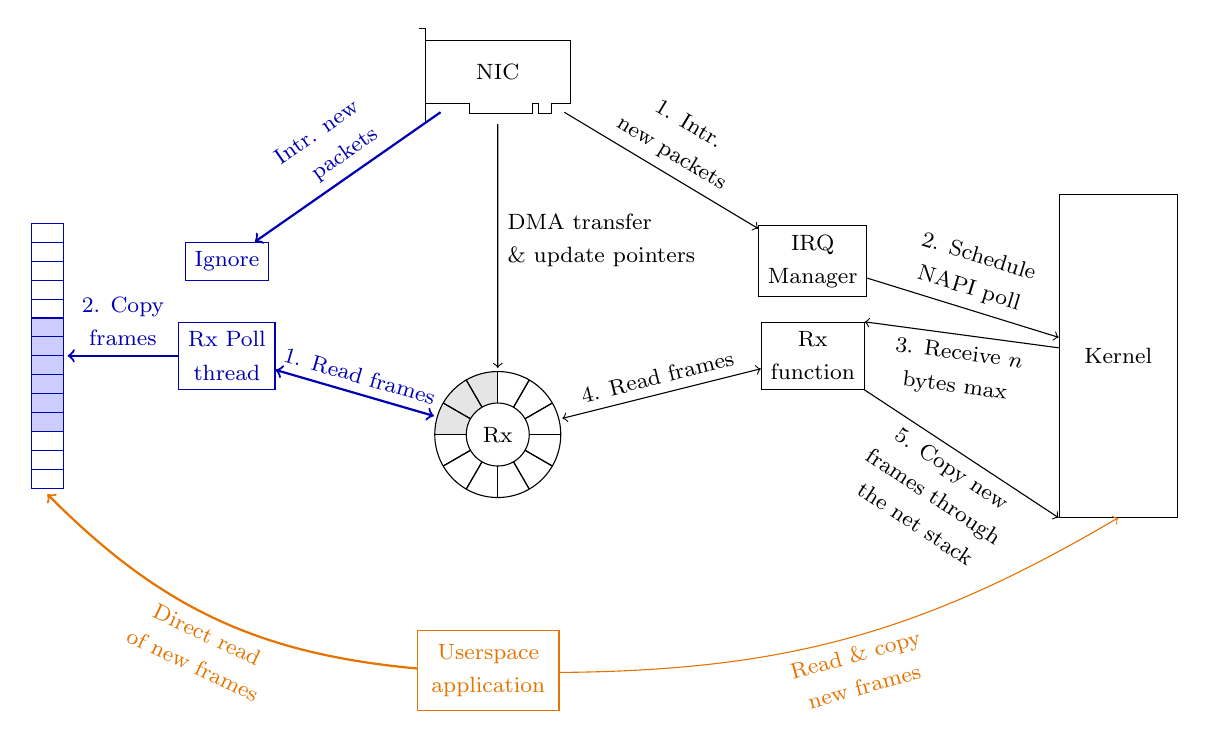
\begin{tikzpicture}[font = {\fontsize{8pt}{12}\selectfont}, scale = 0.8]
\begin{scope}[xshift = 7cm, yshift = 4cm]
\draw (-0.1, 1.2) -- (0, 1.2) -- (0,-0.3) -- (0,0) -- (0.7,0) -- (0.7,-0.15) -- (1.7, -0.15) -- (1.7, 0) -- (1.8, 0) -- (1.8, -0.15) -- (2, -0.15) -- (2,0) -- (2.3, 0) -- (2.3, 1) -- (0,1);

\node[rectangle, minimum width = 2.3cm, minimum height = 1cm] (NIC) at (1.15, 0.5) {NIC};
\end{scope}
\node[draw, align = center] (IRQ) at (13.15, 1.5) {IRQ \\ Manager};
\node[draw, minimum height = 4.1cm, minimum width = 1.5cm] (KRN) at (18, 0) {Kernel};
\node[draw, align = center] (POLL) at (13.15, 0) {Rx \\ function};

\node[draw, blue!70!black] (HIRQ) at (3.85, 1.5) {Ignore};
\node[draw, blue!70!black, align = center] (HPOLL) at (3.85, 0) {Rx Poll \\ thread};
\node[draw, orange!90!black, align = center, inner sep = 5pt] (APP) at (8, -5) {Userspace \\ application};

\begin{scope}[xshift = 8.15cm, yshift = -1.25cm, rotate = 90]
\fill[gray!20!white] (0,0) -- (0,1) arc (90:0:1cm) -- cycle;
\foreach \x in {0, 30, ..., 360}
	\draw ({cos(\x)}, {sin(\x)}) -- ({-cos(\x)}, {-sin(\x)});
\draw (0,0) circle [radius = 1cm];
\draw[black, fill = white] (0,0) circle [radius = 0.5cm]; % Poor man's \clip for intersecting regions
\node[circle, inner sep = 0.45cm] (RNG) at (0,0) {Rx};
\end{scope}

\begin{scope}[xshift = 1cm, yshift = 0cm]
\fill[blue!20!white] (-0.25, -1.2) rectangle (0.25, 0.6);
\draw[blue!70!black] (-0.25, -2.1) rectangle (0.25, 2.1);
\node[blue!70!black, rectangle, minimum width = 0.5cm, minimum height = 3.5cm] (HBUF) at (0,0) {};
\foreach \x in {-2.1, -1.8, ..., 2.1}
	\draw[blue!70!black] (-0.25, \x) -- (0.25, \x);
\end{scope}


\draw[->] (NIC) -- node[midway, above, align = center, sloped] {1. Intr. \\ new packets} (IRQ);
\draw[thick, ->, blue!70!black] (NIC) -- node[midway, above, sloped, align = right] {Intr. new \\ packets} (HIRQ);
\draw[->] (IRQ) -- node[midway, above, sloped, align = center] {2. Schedule \\ NAPI poll} (KRN);
\draw[->] (KRN) -- node[midway, below, sloped, align = center] {3. Receive $n$ \\ bytes max} (POLL.north east);
\draw[->, shorten <= 0.15cm] (NIC) -- node[midway, right, align = left] {DMA transfer \\ \& update pointers} (RNG);
\draw[<->] (POLL) -- node[midway, above, align = center, sloped] {4. Read frames} (RNG);
\draw[->] (POLL) -- node[midway, below, align = center, sloped] {5. Copy new \\ frames  through \\ the net stack} (KRN.south west);
\draw[thick, <->, blue!70!black] (RNG) -- node[midway, above, sloped] {1. Read frames} (HPOLL);
\draw[->, thick, blue!70!black] (HPOLL) -- node[midway, above, align = center] {2. Copy \\ frames} (HBUF);
\draw[->, orange!90!black, thick] (APP) to[bend left = 20] node[midway, below, sloped, align = center] {Direct read \\ of new frames} (HBUF.south);
\draw[->, orange!90!black] (APP) to[bend right = 15] node[midway, below, sloped, align = center] {Read \& copy \\ new frames} (KRN.south);
\end{tikzpicture}

\caption{Architecture of the \textit{ixgbe} driver (black) and HPCAP (blue), showing the different paths that each use to read frames from the reception ring filled by the network interface card (NIC).}
\label{fig:DriverArch}
\end{figure}

Although V\'ictor Moreno's Master's thesis \cite{MorenoTFM2012} already covers the architecture of the HPCAP driver, the main concepts behind it are explained here.

Usually, the manufacturer's driver (\textit{ixgbe}) works via NAPI, a mixed push/poll approach. When the NIC copies new packets to the host memory via DMA, it sends an interrupt that is managed by the driver, which in turn notifies the NAPI subsystem\footnote{``New API'', a extension in the Linux Kernel designed to improve performance by mitigating intterupts. \href{http://www.linuxfoundation.org/collaborate/workgroups/networking/napi}{Documentation is available online}.}. Then, when the kernel is ready, launches the poll function from \textit{ixgbe} with a certain budget $n$. This function will read up to $n$ bytes from the Rx ring, filled by the NIC asynchonously via DMA, and will send the corresponding packets through the kernel's network stack, so they will end up reaching userspace applications.

However, given the motivation of the HPCAP driver (capture at high rates), most of those steps can be bypassed to allow higher performance. First of all, interrupts are disabled and/or completely ignored. Instead, a poll thread runs continously, checking for new packets in the Rx ring and copying them into a bigger buffer (usually, 1GB or more). When a userspace applications wants to read those frames (either to store them to disk or for further processing) it uses the HPCAP API, which will provide direct read access to that bigger buffer.

This architecture is simpler and avoids an unnecessary copy (from the network stack to the userspace application's buffer). It also avoids the extra latency present in NAPI polling systems, which is very useful to have accurate timestamps.

\section{Driver execution flow}

To serve as an introduction to the driver, we explain how does it work from the moment of initialization.

\subsection{Initialization}

\begin{enumerate}
\item The \fileobj{install\_hpcap.bash} script installs the driver with \textit{insmod}, with the corresponding arguments as configured in the \textit{params.cfg} file.
\item The kernel executes the entry point \codeobj{ixgbe\_init\_module}, in the file \fileobj{ixgbe\_main.c}. In this function, HPCAP code ensures that the options are correct (\codeobj{hpcap\_precheck\_options}) and assigns the interface numbers (see \fref{sec:IfaceNumber}).
\item IXGBE registers itself as a PCI driver.
\item For each compatible PCI device found:
\begin{enumerate}
\item The kernel calls \codeobj{ixgbe\_probe} with the PCI structure, so IXGBE can initialize the device.
\item IXGBE prepares the network devices and other structures.
\item HPCAP assigns to the device the corresponding fixed interface number.
\item The device is configured with the corresponding arguments that were passed to the module with \textit{insmod} (see \codeobj{ixgbe\_check\_options}).
\item HPCAP saves a reference to the IXGBE adapter structure in the \codeobj{adapters} array, in the file \fileobj{driver\_hpcap.c}.
\item IXGBE finalizes the initialization of the device (hardware init, network device registration, etc).
\end{enumerate}
\item After IXGBE has finished with the initialization of all devices, \codeobj{hpcap\_register\_adapters} (file \fileobj{driver\_hpcap.c}) is called. For each device working in HPCAP mode, the function \codeobj{hpcap\_register\_chardev} is called. This function does the following:
\begin{enumerate}
\item Creates the \codeobj{hpcap\_buf} structure and saves it in the IXGBE device structure.
\item Registers the character device (see \fref{sec:Chardev}) with the system. This character device will be used for the communication with user-space.
\end{enumerate}
\item After the module has been initialized, Linux wakes up the network interfaces, calling \codeobj{ixgbe\_open}. IXGBE prepares its private configuration, and then calls \codeobj{hpcap\_launch\_poll\_threads} if the interface is in HPCAP mode. This functions ensures that the interface is named correctly (see the corresponding bug description in \fref{sec:bugs:IfaceRenaming}) and then launches the RX poll thread. This thread just copies the new buffers from the NIC ring to the internal HPCAP buffer (see \fref{fig:DriverArch}) if there is a listener. See the ssubsection below for a description of traffic reception.
\item If there are hugepages configured, the \textit{install\_hpcap.bash} scripts allocates and registers them with the system. See \fref{sec:Hugepages}.
\end{enumerate}

\subsection{Traffic reception - kernel side}

The traffic reception is divided in two sections: first, how does the driver receive the data and then how does a client application read it. All the functions for this are defined in \fileobj{hpcap\_rx.c}.

The entry point for the RX thread is \codeobj{hpcap\_poll}. This function loops continously until it is requested to stop. In each iteration:

\begin{enumerate}
\item Checks whether there are client applications reading the traffic. If there are no clients, the read/write offsets are reset (see bug \ref{sec:bugs:CorruptedCapture}) to avoid unaligned memory access.
\item Calls the reception function \codeobj{hpcap\_rx}. While the NIC ring is non-empty, it copies new frames to the internal HPCAP buffer. This function ends when the NIC ring is empty or the internal buffer is filled.
\item Updates the listeners write pointers to notify them of the new data available, calling \codeobj{hpcap\_push\_all\_listeners}.
\item Updates the global read offset according to the slowest listener. Thus the new global read offset will point to the last byte read by all listeners. All the bytes between the write offset and the read offset (take into account that the HPCAP buffer is circular) are ready to be written to with new data.
\end{enumerate}

\subsection{Traffic reception - userspace side}

\begin{enumerate}
\item A client application, such as \textit{hpcapdd} or \textit{monitor\_flujos}, is launched.
\item The client opens the HPCAP character device \textit{/dev/hpcap\_N\_Q} calling \codeobj{hpcap\_open} in \fileobj{libhpcap.c}. This opens the character device with the standard Linux call \texttt{open}.
\item The kernel calls \codeobj{hpcap\_open} in \fileobj{hpcap\_cdev.c}, notifying the driver of the new client. HPCAP assigns it a fixed ID and registers the corresponding listener.
\item The client application maps the HPCAP buffer into its address space, calling \codeobj{hpcap\_map}, which in turns does an \texttt{ioctl} call that returns the necessary buffer information.
\item The client application calls in a loop to \codeobj{hpcap\_ack\_wait\_timeout}, acknowledging how many bytes as it read (this updates the listener read offsets) and updating the count of available bytes (updating its write offset). Then, it can process the new frames, reading them from the previously mapped buffer.
\item Once everything has finished, the client applications closes the HPCAP handle to allow the driver to free the allocated resources and structures.
\end{enumerate}

\section{Character device}
\label{sec:Chardev}

As it has been mentioned in the previous section, HPCAP uses character devices to manage the communication between client applications and the driver. Each interface gets assigned a file \textit{/dev/hpcap\_N\_Q}, where \textit{N} is the interface number and \textit{Q} the queue number\footnote{The queue number is usually 0, as the driver does not correctly support more than one queue.}.

The use of a character device allows the driver to bypass the system's network stack, and gives client applications raw access to the buffer where all the new frames are copied. It also allows using arbitrary \texttt{ioctl} calls, easier to develop and manage, to control the driver. For example, the assignment of hugepages (\fref{sec:Hugepages}) is done via \texttt{ioctl} calls.

\section{Hugepages}
\label{sec:Hugepages}
\index{Hugepage}
To improve performance, the HPCAP driver supports the use of huge memory pages: each adapter may replace its regular buffer by a \textit{hugepage}-backed one. This allows the use of bigger buffers, so traffic peaks can be accommodated easily.

The applications do not need to change anything in order to use \textit{hugepage}-backed buffers. The only required actions are done automatically by the installation script.

The next paragraphs describe the inner workings of the \textit{hugepage}-backed buffer.

\begin{figure}[hbtp]
\centering
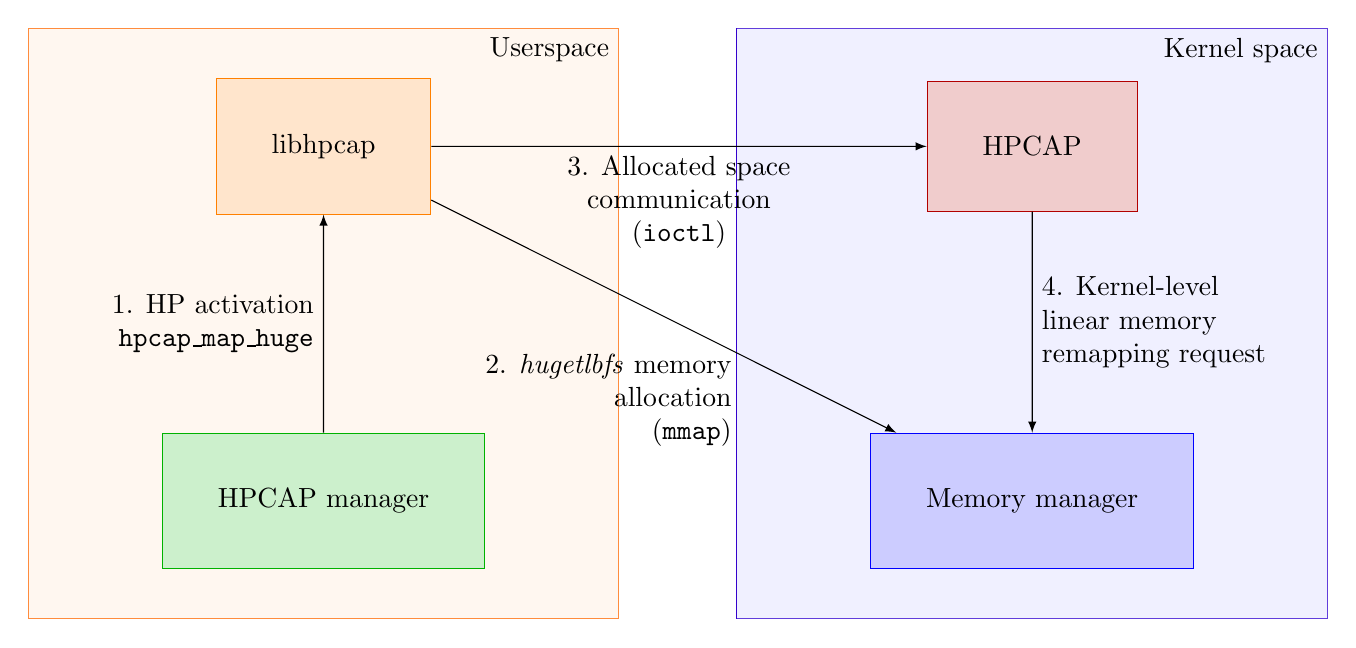
\begin{tikzpicture}[scale=1.5]
\tikzset{>=latex}
\pgfmathsetmacro{\uswidth}{5}
\pgfmathsetmacro{\usheight}{5}
\pgfmathsetmacro{\usyoffset}{\usheight / 2}
\begin{scope}[yshift=-\usyoffset cm]

\coordinate (topright-us) at (\uswidth, \usheight);
\draw[orange!80!red] (0,0) -| (topright-us);
\draw[orange!80!red] (0,0) |- (topright-us);
\fill[orange!20!white, fill opacity=0.3] (0,0) rectangle (topright-us);
\node[anchor = north east] at (topright-us) {Userspace};

\node[orange, fill=orange!20!white, draw, inner sep=20pt, text = black] (lib) at (\uswidth / 2, \usheight - 1) {libhpcap};
\node[green!70!black, fill=green!70!black!20!white, draw, inner sep=20pt, text = black] (manager) at (\uswidth/2, 1) {HPCAP manager};

\draw[->] (manager) -- node[midway, left, align=right] {1. HP activation \\ \texttt{hpcap\_map\_huge}} (lib);

\end{scope}
\pgfmathsetmacro{\scopeoffset}{\uswidth * 1.2}
\pgfmathsetmacro{\kswidth}{5}
\pgfmathsetmacro{\ksheight}{5}
\pgfmathsetmacro{\ksyoffset}{\ksheight/2}
\begin{scope}[xshift=\scopeoffset cm, yshift=-\ksyoffset cm]
\coordinate (topright-ks) at (\kswidth, \ksheight);
\draw[blue!80!red] (0,0) -| (topright-ks);
\draw[blue!80!red] (0,0) |- (topright-ks);
\fill[blue!20!white, fill opacity=0.3] (0,0) rectangle (topright-ks);
\node[anchor = north east] at (topright-ks) {Kernel space};

\node[blue, fill=blue!20!white, draw, inner sep=20pt, text = black] (kernmem) at (\kswidth / 2, 1) {Memory manager};

\draw[->] (lib) -- node[midway, below, align=right, xshift=-20, yshift=-10] {2. \textit{hugetlbfs} memory \\ allocation \\ (\texttt{mmap})} (kernmem) ;

\node[red!70!black, fill=red!70!black!20!white, draw, inner sep=20pt, text = black] (hpcap) at (\kswidth /2, \ksheight - 1) {HPCAP};

\draw[->] (lib) -- node[midway, below, align=center] {3. Allocated space \\ communication \\ (\texttt{ioctl})} (hpcap);

\draw[->] (hpcap) -- node[midway, right, align=left] {4. Kernel-level \\ linear memory \\ remapping request} (kernmem);
\end{scope}

\end{tikzpicture}
\caption{Schematic of the hugepage allocation and buffer assignment to the driver.}
\label{fig:HPCAPMapping}
\end{figure}

To use the driver with hugepages, first it should be activated calling the function \texttt{hpcap\_map\_huge}. The \fileobj{huge\_map} application, in the \textit{samples} folder (see \fref{sec:samples:hugemap}), does this call easily from user-space. The install script \texttt{install\_hpcap.bash} does this automatically when an interface is configured in mode 3 (although the mode is always 2 in the buffer).

Once the call to \texttt{hpcap\_map\_huge} is done, the \textit{libhpcap} library takes control. The function \texttt{\_hpcap\_mmap\_hugetlb} will get a memory region of the requested size backed by the system's hugepages. In order to do this, it will create a file in the \textit{hugetlbfs}\footnote{See \fref{sec:hugepages:hugetlbfs} for a description of the \textit{hugetlbfs} filesystem.} filesystem and will call \texttt{mmap} to obtain the memory address.

Once the memory region pointer has been obtained, it will be transferred to the HPCAP driver by means of a \texttt{ioctl} call. The \texttt{ioctl} controller in the driver will call \texttt{\_hpcap\_use\_huge}. This function will obtain from the kernel the actual pages that make up the buffer.

A small trick used when calculating the number of pages, is that the page size used is not 1GB (or whatever is the hugepage size in the system), but the default regular page size of the system (4KB usually). Despite this, the pages used will actually be \textit{huge pages}.

The kernel function \codeobj{get\_user\_pages} will be called with the page number calculated as explained. Here, a problem may occur. When the buffer size is greater than the \textit{hugepage} size, the pages returned may be unordered and memory addresses will not be sequential\footnote{See \href{http://stackoverflow.com/questions/25000494/sequential-access-to-hugepages-in-kernel-driver}{this StackOverflow} question for further discussion of the problem and solution.}. To solve this, \codeobj{vm\_map\_ram} is called, obtaining a virtual address that can be accessed sequentially.

Once the buffer address is ready, the buffer of the given adapter is replaced by the \textit{hugepage}-backed one. Additionally, certain parameters are saved in the adapter structure in order to manage and free the buffer later.

\subsection{Releasing \textit{hugepage} resources}

There are several parts of the system where references to the \textit{hugepages} buffer are kept:

\begin{itemize}[itemsep = 0pt]
\item Kernel driver.
\item Userspace applications that allocated the buffer and transferred it to the driver.
\item Userspace applications that map the adapter memory.
\item \textit{hugetlbfs} filesystem.
\end{itemize}

In order for the memory to be freed, no references should be left.

The application allocating the \textit{hugepages} buffer loses the references once it is closed. The applications calling \texttt{mmap} lose them in the same way, although the handles can be released by calling \codeobj{munmap}.

The driver releases the references once the adapters are unregistered, which can happen on module unloading or when changing the adapter configuration.

The references in the \textit{hugetlbfs} filesystem are deleted when calling \codeobj{hpcap\_unmap\_huge}. If they are still present, they can be released simply by deleting the corresponding files in the filesystem.

To see the statistics of the system's hugepages, you can use the \codeobj{hp\_info} function in the \fileobj{hpcap-lib.bash} script. Just source that file in your shell (\texttt{source scripts/lib.bash}) and call \texttt{hp\_info} to see the statistics. This function just extracts the information from the \fileobj{/proc/meminfo} file.

\subsection{\textit{hugetlbfs} filesystem}
\label{sec:hugepages:hugetlbfs}

As explained in the \href{https://www.kernel.org/doc/Documentation/vm/hugetlbpage.txt}{kernel docs}, an easy way to access and use \textit{hugepages} is via the \sysobj{hugetlbfs} filesystem. This is a virtual filesystem that can be accessed as any other part of the Linux folder tree. It is mounted with the \sysobj{mount} application:

\termcommand{mount -t hugetlbfs none /mnt/hugetlb}

The \textit{hugetlbfs} accepts several parameters, documented in the \href{https://www.kernel.org/doc/Documentation/vm/hugetlbpage.txt}{kernel docs}:

\termcommand{mount -t hugetlbfs -o uid=<value>,gid=<value>,mode=<value>,size=<value>,nr\_inodes=<value> none <hugetlfs\_path>}

Files created inside this filesystem are, from the user point of view, the same as every other file in the system. However, under the hood, these files are pointers to memory regions backed by \textit{hugepages}. That means that if they are mapped with a call to \texttt{mmap}, what will be returned will be a pointer to a \textit{hugepage}-backed memory buffer.

In order to use hugepages, your system must me configured properly at boot time. That means that you should add the corresponding parameters to the \textit{linux} command in your \textit{grub.cfg} file. These parameters are \textit{default\_hugepagesz, hugepagesz} and \textit{hugepages}, as documented in the kernel documentation. For example, the parameters \texttt{default\_hugepagesz=1G hugepagesz=1G hugepages=8} would enable hugepages of 1 GB, and then would allocate 8 hugepages of 1GB at boot time. In the end, your \textit{linux} boot command could look like this:

\texttt{linux /boot/vmlinuz-3.8.0-29-generic root=UUID=b2be13dc-7a60-4928-b61a-cc3ec95044a0 iommu=pt intel\_iommu=on isolcpus=0,1,2,3,4,5 ro default\_hugepagesz=1G hugepagesz=1G hugepages=8}

To make the hugepage mounting process easier, the script \fileobj{hugepage\_mount} in the \textit{scripts} directory will mount the \textit{hugetlbfs} filesystem in the default path \textit{/mnt/hugetlb} if no \textit{hugetlbfs} filesystem is already mounted. It will also detect when the system does not have hugepages activated.

\section{\texttt{ioctl} interface}

To allow communication between client (userspace) applications and the driver, the \codeobj{ioctl} system call is used.

For listener operations (acknowledging read bytes or waiting for new data to arrive), the \texttt{ioctl} code used is \codeobj{HPCAP\_IOC\_LSTOP}, that sends a \codeobj{hpcap\_listener\_op} structure with all the data. The driver will receive that structure and do the necessary operations. Refer to the code in \fileobj{hpcap\_cdev.c} for details.

For buffer operations (buffer information and hugepage mapping (\fref{sec:Hugepages})), the structure used is \codeobj{hpcap\_buffer\_info}. The operation to perform will be decided depending on the \texttt{ioctl} command used. The relevant operations are \codeobj{HPCAP\_IOC\_BUFINFO}, \codeobj{HPCAP\_IOC\_HUGE\_MAP} and \codeobj{HPCAP\_IOC\_HUGE\_UNMAP}. Again, refer to the code in \fileobj{hpcap\_cdev.c} for details on how are these commands processed.

\subsection{\texttt{ioctl} version compatibility}

When changing the structures and \texttt{ioctl} commands, client applications compiled for previous versions may fail and, what's worse, do it without a easy-to-understand error message. To avoid this problem, apart from documentation and version number changes\footnote{As \fref{sec:versioning} explains, backwards-incompatible changes such as changing the \texttt{ioctl} commands and/or arguments should reflect in an increase in the major version number.}, the magic number (\codeobj{HPCAP\_IOC\_MAGIC}) should be updated to stop old versions from issuing commands that the new driver will see as corrupted.

The other option (adding a version check field to the structure) was actually implemented in commit 4aba154098fe5d12019d4c65e7be477a98ad8735, but reverted later after it was noticed that increasing the magic number would have the same results, better reliablity and less complexity. If you want to go back to the version check field, just revert the revert commit (dc01554a5220d32d947ab9eedead03736d526805).

\section{Interface numbering}
\label{sec:IfaceNumber}

The HPCAP interfaces receive a fixed name based on the PCI bus ID, to avoid renamings after a reboot of the monitoring system. All the functions related to this capability are in the file \fileobj{hpcap\_pci.c}.

To achieve this fixed naming, the \textit{ixgbe} driver first calls \codeobj{hpcap\_fix\_iface\_numbers} with the list of recognized PCI devices. This function searches all devices matching those PCI IDs (that is, all the supported NICs) and assigns them a fixed number. After initialization, HPCAP will call to the other functions in the file to retrieve the fixed numbers assigned.


\section{Debugging \& testing}

In this section we will describe several techniques to debug and test the HPCAP driver. Take into account that there are no debuggers like \textit{gdb} (or at least they're not that useful).

\subsection{Traffic generation}

Usually, the first issue that appears when testing the driver is the need for generating traffic at high rates. There are several solutions, most based on Intel DPDK (Data Plane Development Kit).

To install DPDK, you should \href{http://dpdk.org/download}{download it} and uncompress it, and then follow these steps:

\begin{enumerate}[itemsep=0pt]
\item In the \textit{dpdk} folder, go to \textit{tools} and run \textit{setup.sh} as root. A menu will appear.
\item Select the appropiate build option for your architecture (probably \textit{x86\_64-native-linuxapp-gcc}).
\item Set up the hugepage mappings for your architecture (NUMA/non-NUMA). I usually choose 1024 pages, but it is a flexible parameter.
\item Insert the IGB UIO module (for Intel IXGBE NICs).
\item Bind the desired Ethernet devices to the IGB UIO module. The ethernet devices appear with the PCI bus number and the interface they're bound to. If you want to bind an active interface (marked with \textit{*active*}), first bring it down with \texttt{ifconfig iface down}. If you are not sure which interface corresponds to each physical link, you can use \texttt{ethtool -p iface} to make the LED lights on the corresponding physical interface blink for easy identification.
\end{enumerate}

Now, the available traffic generators.

\subsubsection{pktgen-DPDK}

\index{DPDK} \href{http://dpdk.org/download}{pktgen-DPDK} is a packet generator based on DPDK, very flexible but sometimes not predictable and not too easy to start configure.

To build it, you should build DPDK as explained above (even if it's already built) and then, in the same terminal session, run \texttt{make} in the \textit{pktgen-dpdk} folder. If DPDK is not built, some environment variables are not exported and the pktgen compilation will fail.

Once compiled, you can run it with a command line such as this one:
\begin{verbatim}
./app/app/x86_64-native-linuxapp-gcc/pktgen -c FF -n 4 -- -T -P -m "[1-7:1].0"
\end{verbatim}

These arguments are separated on two sections: the part before the \texttt{--} is related to DPDK and its ``EAL'' options. The \texttt{-c FF} is the core mask, and selects the cores to use. In this case, \texttt{FF = 1111 1111}, that is, use all 8 cores. \texttt{FE = 1111 1110} would use only 7, although it is not clear which core (the first or the last one) is unselected. The \texttt{-n 4} is the number of memory channels to use. More gives better performance, but there's usually a limit on how many can be used.

For the \textit{pktgen} options (the part after the \texttt{--}), \texttt{-T} gives colored output, \texttt{-P} enables promiscous mode and, the most important part, the \texttt{-m "[1-7].0"} defines the core assignment. In this case, it assigns cores 1 to 7 to the interface 0. Running \texttt{pktgen --help} will give more examples of the syntax, just remember to keep all the specifiers between quotes. A tip: the first core (0) is usually assigned to the display thread, so assigning it to an interface could make the program fail.

When the core assignment is not correct, \textit{pktgen} does not show an error message, it just stops. However, in the middle of all the output it produces there's a table with the cores and ports: if it's empty, you know your core assignment was wrong.

Once \textit{pktgen} starts, it has a nice interface where you can configure the generator. Typing \texttt{help} will describe all the available options, including changing the IP or MAC destination.

For a quick start, set the frame size with \texttt{set [port-number] size X} and the rate with \texttt{set [port-number] rate R}, where \texttt{R} is a percentage between 0 and 100: actual transmission rate will be the $R \%$ of the maximum rate of the port. Then, start the transmission with \texttt{start [port-number]}. In all of the previous commands, \texttt{port-number} can be \textit{all} to act on all the available ports at the same time.

If you want to send PCAP files with \textit{pktgen-DPDK}, you have to add arguments to the command line and then activate the PCAP sending in the interface\footnote{And have a little bit of luck. We have not been able to test this feature as it requires a huge amount of memory (the allocations are not efficient at all).}. The command line arguments should look like this: \texttt{-s I:path}, where \texttt{I} is the index of the port from which you want to send the PCAP, and \texttt{path} is the path of the PCAP file. Once \textit{pktgen-DPDK} has started, activate the PCAP sending with \texttt{pcap [port-number] enable}.

\subsubsection{MoonGen}

\index{MoonGen} \href{https://github.com/emmericp/MoonGen}{MoonGen}, also based on DPDK, is a packet generator specialized in scripting. It uses Lua as an scripting language, is fast and more predictable than \textit{pktgen}, but less useful if you just want to do a quick test. The \href{https://github.com/emmericp/MoonGen#installation}{installation instructions} on its page are complete.

This is the generator used for automated testing. There's a script in the HPCAP folder, \textit{scripts/fixed-rate.lua}, which can generate traffic at a fixed rate with custom frame sizes. It can be used as a base for writing other scripts for MoonGen. Their \href{http://scholzd.github.io/MoonGen/index.html}{API documentation} is also decent.

\subsection{ethtool counters}

It's really easy to add new counters that will show up with \sysobj{ethtool} when running \texttt{ethtool -S hpcapX}. In the file \fileobj{ixgbe\_ethtool.c}, modify the \codeobj{ixgbe\_gstrings\_stats} and add new entries. These entries need to have a string identifying the counter, and the corresponding field in the \codeobj{ixgbe\_adapter} structure. You should only worry about modifying that field when appropiate: the \textit{driver} will take care of transmitting that information to the \textit{ethtool} system.

Currently, there are two extra counters in \textit{ethtool}: \texttt{rx\_hpcap\_client\_lost\_frames} and \texttt{rx\_hpcap\_noclient\_frames}. The first one marks the frames that were discarded because the intermediate buffer was full. The second one counts the frames discarded because there were no clients ready to receive them. Note that these counters are note 100\% precise and may not count all the losses of the driver: it is expected behaviour, as the driver will exit the reception loop when it is not able to copy the packets to the intermediate buffer.

\subsection{Automated testing}
\label{sec:debugtest:AutomatedTesting}

In order to make testing easier, a script for automation is provided: \fileobj{scripts/hpcap-test}. The test parameters (e.g., generator port, generator host, traffic rates or tests to execute) can be configured in the file \fileobj{hpcap-test.cfg} (you can create it renaming \textit{hpcap-test.cfg.sample}). All the options are documented in the configuration file.

The test script ensures that the driver, samples and libraries compile correctly, that the driver can be installed and removed from the system without problems and with a coherent status, and then starts with extra tests.

These extra tests are located in the \fileobj{scripts/tests} folder. To add new tests, the only thing needed is to create another file in that folder, and to activate the corresponding test in the configuration file, adding an option \texttt{test\_filename=true} in the \fileobj{hpcap-test.cfg}, where \texttt{filename} is the name of the file that was just created in the \textit{scripts/tests} folder.

The tests can use functions defined in the \textit{scripts/hpcap-test} file, such as \texttt{reinstall\_hpcap} or \texttt{install\_hpcap}; \texttt{begin\_test, test\_ok, test\_fail} to mark the beginning and results of a test and \texttt{test\_fail\_die} to mark the test as failed and aborting the session (for example, when the driver is corrupted or any other thing goes horribly wrong).

The functions in \textit{scripts/hpcap-lib.bash} can also be used. Of special interest are \texttt{start\_generator}, which receives as arguments the generation rate in Mbps and the frame size and starts the traffic generator in the background; and \texttt{stop\_generator} whose result is obvious.

All of the configuration of the test (e.g. receiver interface, generator configuration) is read from the \fileobj{hpcap-test.cfg} file, in bash-like format. Most options are documented in the file. All the variables are read and are available with the same name in all of the test scripts.

\subsubsection{Test cases}

Apart from the basic test cases described above, the following extra tests are available:

\begin{itemize}
\item \textbf{bad\_padding}: Tests for a edge case in the padding insertion, where the space left in the current file is exactly the size of a RAW header. This test was written to ensure that bug \ref{sec:bugs:AllFramesLost} did not appear again.
\item \textbf{small\_buffer}: A test of reception with small-ish buffers, not using hugepages. This may discover issues with overflowing counters.
\item \textbf{traffic\_rx}: Tests that the driver can support a high rate of reception without losses. All the traffic is discarded by \textit{hpcapdd}.
\item \textbf{traffic\_store}: Tests whether the driver can support a decent rate of traffic reception without losses while saving the traffic to disk. Also ensures that the generated RAW files are correct and there's no malformation.
\end{itemize}

All of the parametres of these tests can be configured in the same \textit{hpcap-test.cfg} files.

\subsection{\textit{Post-mortem} debugging}

When the driver crashes or stops working, there are several options to try and see what has happened. We will see them from best-case to worst-case.

The best case occurs when the driver does not work appropiately but it is still loaded in the system and responding to some commands. The kernel log (run \texttt{dmesg -H}) may show error messages that may or may not give some clues. If you want extra information about the driver, installing a debug build (\texttt{make debug; ./install\_hpcap.bash bin/debug/hpcap.ko}) will show more messages (make sure of enabling the messages for the categories you need in \fileobj{driver/common/hpcap\_debug.h}, see next \fref{sec:debugtest:macros}) that may help.

The application \textit{statusinfo} can also be used to show information about a HPCAP interface in the console, such as read/write offsets, connected listeners and thread states. It is pretty useful when the driver has stopped receiving traffic but there are no messages telling why, and a debug build cannot be installed.

The next case is when the driver stops working and crashes but does not crash the system. Usually, there's a backtrace in the kernel log that shows the address of the instruction that crashed, although in hexadecimal format (e.g., \texttt{hpcap\_rx+0x32c/0x660}), which is not very useful. \textit{addr2line} can be used to see the actual line in the file, but usually \textit{gdb} is more reliable. Run \texttt{gdb bin/debug/hpcap.ko}, making sure that the binary is the same that was installed when the crash happened. Then, the command \texttt{l *(hpcap\_rx+0x32c/0x660)} will show the exact file and line of the instruction that crashed the driver.

The worst case (and also the common one) is that the driver crashes and takes the system with it. If the \sysobj{kdump} service is enabled, the memory image and the \textit{dmesg} log are saved to \textit{/var/crash}, which can be useful to see what happened. See your distribution's instructions on how to enable \textit{kdump}\index{kdump} (e.g., \href{https://fedoraproject.org/wiki/How_to_use_kdump_to_debug_kernel_crashes}{this for RedHat based distros}).

\subsection{Diagnostic collection tool}

To facilitate the diagnosis of failures and bugs in production environments, the script \fileobj{scripts/diagnostics} can be used to collect information that can help to discover what happened. After collection, the tool generates a \textit{.tar.gz} compressed file so it can be easily sent by mail or any other means.

Currently, this script collects the following information:

\begin{itemize}[itemsep=0pt]
\item \textbf{System information}: Installation path, kernel version, distribution version, PCI deices, kernel modules installed, mounted filesystems, system topology, CPU information, memory information, running processes and kernel log.
\item \textbf{Crash logs}: Crash logs stored in \textit{/var/crash}. Not very useful if the system does not have \textit{kdump} enabled\footnote{See \href{https://fedoraproject.org/wiki/How_to_use_kdump_to_debug_kernel_crashes}{this for RedHat based distros}.}.
\item \textbf{HPCAP information}: Configuration, driver version, driver modinfo, installation status and monitor logs.
\item \textbf{HPCAP interfaces data}: ifconfig and ethtool output, ethtool statistics, listener status and character devices.
\item \textbf{Capture information}: Size and location of all capture files (the search path is the filesystem root, excluding system folders such as \textit{/etc, /home, /usr}, ...).
\end{itemize}

\subsection{Outputting debug information to the kernel log}
\label{sec:debugtest:macros}

There are several macros that facilitate the output of debug information. These are defined in the file \fileobj{hpcap\_debug.h}. All print the corresponding driver prefix (defined in the \codeobj{PFX} macro, containing \textit{ixgbe} or \textit{ixgbevf} depending on the driver) to allow their identification in the kernel log.

\begin{itemize}
\itemdesctt{printdbg} Enabled only in \textit{debug} configurations. Prints the information along with the tag ``dbg'' and the currently executing function.
\itemdesctt{adapter\_dbg} Enabled only in \textit{debug} configurations. Prints the same output that \texttt{printdbg}, but includes the current adapter name. This information is retrieved from the \textit{adapter} variable.
\itemdesctt{bufp\_dbg} Enabled only in \textit{debug} configurations. Prints the same output that \texttt{printdbg}, but includes the current buffer (adapter and queue). This information is retrieved from the \textit{bufp} variable.
\itemdesctt{BPRINTK} Basic kernel printing with the corresponding prefix and current function.
\itemdesctt{HPRINTK} Kernel printing with the corresponding prefix, current function and current buffer (adapter and queue). This information is retrieved from the \textit{bufp} variable.
\itemdesctt{DPRINTK} Kernel printing with the corresponding prefix and current function, including adapter name. It also prints to the network interface log.
\end{itemize}

The question of which function to use is easy. If you want to print a debug statement use the \texttt{dbg} functions, preferably \texttt{adapter\_dbg} if the \textit{adapter} variable is accessible. If the statement should always be printed in the kernel log, even in production releases, use the \texttt{XPRINTK} variant that outputs all the information you have in the current scope. That is, \texttt{DPRINTK} if the \textit{adapter} variable is in the scope, \texttt{HPRINTK} if we have \textit{bufp}, or else use \texttt{BPRINTK}.

The \textit{dbg} variants (\texttt{printdbg, adapter\_dbg, bufp\_dbg}) all receive a first argument that describes the type of debug statement. This should be one of the \texttt{DBG\_XXX} macro that allows control of which kind of statements get printed out.

% -*- root: ../HPCAP_DevGuide.tex -*-
\section{Bugs, system errors and known issues}
\label{sec:bugs}

This section shows the bugs that have been found during the development and use of the driver, hoping that it gives the reader some ideas when the driver and/or the kernel have turned crazy and decided not to work.

\subsection{Driver/system corruption after system crash}
\label{sec:bugs:drivercorrupt}

\begin{bugdata}
\bugfixed[06b9ec8: insmod: Blacklist hpcap and ixgbe to avoid loading them at unusual times
]
\versions{4.2.0, 4.2.1}
\end{bugdata}

During the testing of HPCAP 4.2.1, the system crashed because of unknown issues while HPCAP was receiving traffic. The driver was installed to the system. After a reboot, something was corrupted: both \textit{ixgbe} and \textit{hpcap} were loaded at boot (even though none of them was configured to do so) and could not be removed. Trying to install the module again resulted in either errors or \textit{modprobe/insmod} hanging.

It seems that, after a crash, the Linux kernel tries to reload the modules in some weird fashion, reloading both \textit{ixgbe} and \textit{hpcap} and causing some weird conflicts, including errors in the Intel Direct Cache Access subsystem (in some instances, the driver crashed on install with the stack trace pointing to \texttt{dca\_register\_notify}).

% Comment to facilitate searching: dca_register_notify

The fix was to blacklist both drivers in the \textit{modprobe} configuration that was already being generated on install. When the error happened, the system could be restored running \texttt{depmod -a \&\& update-initramfs -u} with \textit{root} permissions, or reinstalling the kernel.

\subsection{Segmentation fault on client applications}

\begin{bugdata}
\bugfixed[9f21f1f: Fix concurrency issue when adding listeners]
\versions{4.1.0 and previous}
\end{bugdata}

Sometimes, when multiple clients open the same HPCAP handle at the same time (for example, \sysobj{monitor\_flujos} opens two handles on the same file), a race condition may occur and the listener identifications will not be registered correctly. This causes messages in the kernel log warning about some ``listener not found'' and possibly a segmentation fault when issuing \texttt{ioctl} calls. The solution was to properly protect critical sections of the code that can be read and written concurrently.

\subsection{modprobe/insmod: Cannot allocate memory}

\begin{bugdata}
\bugnotfixed
\versions{All}
\end{bugdata}

There are several possible causes. If the error is raised by the HPCAP driver, you should see a line in the kernel log explaining what happened and how to correct the error\footnote{If the message appears but does not tell how to fix the error or does not explain what's happening, tell the maintainer to change that error message.}.

However, if the kernel log doesn't show any message from \textit{hpcap}, it may be an issue with available memory in the kernel. The Linux kernel has a certain memory space assigned to load modules\footnote{See \href{https://www.kernel.org/doc/Documentation/x86/x86_64/mm.txt}{the kernel documentation about the matter}.}, usually about 1.5GB. It's more than enough for regular uses of modules, but not in the case of HPCAP. HPCAP allocates a static buffer of 1GB that will be shared between the different queues. This buffer is placed on that module mapping space\footnote{It may be possible that I'm wrong here about this.} so, if several modules have already reserved more than 500 MB, the kernel may refuse to load our module.

The workaround for this is to reduce the buffer size (modify the macro \codeobj{HPCAP\_BUF\_SIZE} in the \fileobj{include/hpcap.h} file) and, if necessary, to use hugepages (see \fref{sec:Hugepages}) to get buffers of the necessary size. I haven't found any way to see the memory usage of each driver nor how to see how much of that module mapping space is already allocated.

\subsection{Interfaces renamed automatically by udev}
\label{sec:bugs:IfaceRenaming}

\begin{bugdata}
\bugfixed[r715: insmod: workaround for udev renaming rules, r807]
\versions{4.2.2 and previous}
\end{bugdata}

In some systems, udev has some ``smart'' renaming rules \href{http://www.freedesktop.org/wiki/Software/systemd/PredictableNetworkInterfaceNames/}{that theoretically gives a predictable naming to the network interfaces}. That interferes heavily with HPCAP. The workaround consists in a small check in the \codeobj{interface\_up\_hpcap} bash function, that will check in the kernel log for \textit{udev} renamings and will undo them.

An extra problem in some CentOS installations was that \textit{udev} did not even print in the kernel log these renames. This required an extra fix (revision 807 in \textit{mellanox} branch, merged into trunk in rev. 838), that consisted of a naming check (the actual function is called \codeobj{hpcap\_check\_naming}) that is called before launching the poll threads. This functions compares the current name of the interface to the expected one (\textit{hpcapX}, where \textit{X} is the adapter index): if they are different, it prints a message to the kernel log that will be picked up by the installation script so it can rename the interfaces.

\subsection{Corrupted capture files}
\label{sec:bugs:CorruptedCapture}

\begin{bugdata}
\bugfixed[r842, r869]
\versions{4.2.3 and previous}
\end{bugdata}

A bug was discovered where the captures were being corrupted if another program had been listening previously. For example, if a first instance of \textit{hpcapdd} was launched and then closed, the resulting capture files were all correct. However, if a second instance was launched without reinstalling the drivers, all capture files would be corrupted.

The actual issue had to to with how the clients (listeners) acquire their reading offsets. A first listener would start reading from offset 0, transferring blocks of a fixed size. When the client closed, HPCAP saved the last reading offset, which would not necessarily point to the beginning of a frame.

Thus, when another new client tried to read from the HPCAP buffer, its reading offset was the last reading offset of the other client. This new client would begin saving the capture at the middle of a frame, so applications such as \textit{raw2pcap}, expecting to read first a correct packet header, would crash and/or output completely wrong results.

A first solution was to assign as read offset the last writing offset of the HPCAP producer. New frames are written starting from that offset, so new listeners would start reading frames with the correct headers. However, this caused another extra problem: misaligned access to the buffer that could hurt performance. A fix for this issue is simply resetting the read/write offsets when there are no listeners: if there are no client applications, HPCAP will forget the last read/write offsets and will start writing frames from offset 0, thus avoiding misaligned access for new clients.

A secondary bug appeared later, introduced by the first fix (r842): in some cases the global write offset would be advanced before the read offset of a new listener was configured. In these cases, the read offset would again be greater than 0 and would cause errors when writing the captures. This bug was fized in r869 by setting the read/write offsets in the intialization of the listener.

\subsection{Connection failure / segfault on xgb interfaces}

\begin{bugdata}
\bugfixed[r826: ixgbe: Fix bug with ixgbe interfaces where next\_to\_use wasn't being updated and caused errors]
\versions{4.2.3. Possibly previous versions, not checked}
\end{bugdata}

Interfaces configured in the \textit{xgb} mode were failing and/or crashing the system completely when they received data.

The cause was that the \texttt{rx\_ring->next\_to\_use} pointer was not updated correctly. It should be updated in \codeobj{ixgbe\_release\_rx\_desc} to have the same value as the ring's tail pointer of the NIC, but the corresponding line was missing. This caused incoherencies between the ring status in software and in hardware, which in turn caused missing frames (thus the failing connections) and even crashes when the software tried to access to unallocated descriptors.

\subsection{Connection reset after TX hang}

\begin{bugdata}
\bugfixed[r875, r876: ixgbe: Disable transmission and forced resets on TX hangs]
\versions{4.2.3 and previous}
\end{bugdata}

If an application in the system tried to send frames through interfaces configured in HPCAP mode, it could trigger a reset in the interface that would lead to corrupted captures.

The bug was that the \textit{ixgbe} driver would store the packets to send in a queue which was not flushed. Then, a watchdog (either in the driver or in the kernel) would notice\footnote{The exact message was \textit{initiating reset due to lost link with pending Tx work}.} and reset the adapter. This would in turn reset the poll thread and corrupt the capture.

The solution was to discard frames to transmit in HPCAP adapters, and to disable the code that resets the adapter when using HPCAP work modes.

\subsection{Loss of all frames}
\label{sec:bugs:AllFramesLost}

\begin{bugdata}
\bugfixed[r963: hpcap: Fix bug where the driver was losing all frames]
\end{bugdata}

A misterious bug where at random times caused the driver to lose all frames. The cause was the padding check. When receiving a packet, if the space left in the capture file was exactly 2 RAW headers plus the incoming packet size, no padding would be written. The space left for the next frame was exactly the size of the RAW header, so the padlen, calculated as the remaining space in file \textit{minus the size of a RAW header} would be zero and no padding would be inserted. The file size would be also incremented, surpassing the value of \texttt{HPCAP\_FILESIZE} and either corrupting the memory space when writing with erroneous lengths or avoiding the reception of any packets as the driver would not have space to insert the padding with that size.

\subsection{IOCK and MNG\_VETO bit enabled - capture thread stops}

\begin{bugdata}
\bugnotfixed
\versions{pre-5.0.0, at least}
\end{bugdata}

In a certain installation, the driver would stop capturing after the system received a non-maskable interrupt about an IOCK error. There is not much documentation about this error, but it seems to be related with the hardware.

The kernel log also showed a message from the base \textit{ixgbe} driver about a \texttt{MNG\_VETO}\index{MNG\_VETO} bit enabled. Reading the NIC datasheet \cite{825992010}, it seems to be a bit set up by the hardware when it is in low-power state that forbids link changes, so downed links would not be restored.

As of 27/4/2016, this bug seems to be caused by the hardware.

\subsection{Concurrent listeners leads to losses and/or data corruption}

\begin{bugdata}
\bugfixed[r959, r955]
\versions{4.2.3 and previous}
\end{bugdata}

Several related errors happened when there was more than one client listening for data in a HPCAP interface. For example, if a listener connected first but did not read anything, a second listener would receive an advanced read offset (the last write from the polling thread). So, even when the two listeners could start reading data from the buffer at the same time they would see different data. This was fixed in revision 959.

Another problem happened when two listeners connected to the driver and then the first one disconnected. The next listener to connect would receive handle ID 2, which was already being used. Data loss and/or corruption of the structures would then occur. This was fixed in revision 955.

\subsection{Copies from/to user space can fail}

\begin{bugdata}
\bugfixed[r956: hpcap: Fix copies from/to the user memory]
\versions{4.2.3 and previous}
\end{bugdata}

In the \texttt{ioctl} calls, the copies to and from user space memory were not being done with \texttt{copy\_to/from\_user} and, in strange instances where that memory was invalid, that could cause a segfault within the driver. With the fix, no invalid acceses are done and the correct error message is returned to the caller application.

\subsection{Corrupted capture files after restarting a client}

\begin{bugdata}
\bugfixed[r893: hpcap: Reset written buffer size when there're no listeners]
\versions{4.2.3 and previous}
\end{bugdata}

Related to bug \ref{sec:bugs:CorruptedCapture}, when restarting a listener, the captures would be subtly corrupted as the driver would not place the padding at the end of the file but in the middle instead. This happened because the filesize counter was not being reset if there were no listeners.

\subsection{Problems when using buffers greater than 2GB}

\begin{bugdata}
\bugfixed[r990: hpcap: Fix several problems with buffers greater than 2G]
\versions{4.2.X}
\end{bugdata}

When using hugepage-backed buffers with a size greater than 2GB, several variables would overflow and cause segfaults and memory errors.

There is a secondary problem: when allocating buffers of size 4GB, the function \codeobj{vm\_map\_ram} used in the hugepage code will segfault due to a bug in the Linux kernel code. See \href{http://marc.info/?l=linux-mm&m=146114962421719&w=2}{the linux-mm mailing list} for more information. The patch was included in kernel version 4.7.

\subsection{Frames with VLAN tags disappeared}

\begin{bugdata}
\bugfixed[r1025: ixgbe: Fix VLAN stripping]
\versions{pre-5.0.0}
\end{bugdata}

During the update of the ixgbe base driver from 3.7.17 to 4.1.2, the VLAN stripping features were not correctly deactivated. This caused the card to strip the VLAN tags in hardware. The solution was to disable all hardware features in the correct location in the code.

\subsection{RX Errors with no cause}

\begin{bugdata}
\bugnotfixed
\versions{All}
\end{bugdata}

In some environments, the \textit{ethtool} counters for \texttt{rx\_errors} increment, but without CRC or length errors. These may be caused by corrupted non-Ethernet packets, such as malformed Cisco Spanning Tree Protocol (STP) frames. The solution was to make the NIC stop counting these frames as errors, disabling a certain register. This required to add the line \begin{verbatim}
hlreg0 &= ~IXGBE_HLREG0_RXLNGTHERREN
\end{verbatim} in \textit{ixgbe_main.c:4659}, in the \codeobj{ixgbe\_set\_rx\_buffer\_len} function.


\chapter{NIC Interface and communication}

Refer to the Intel controller datasheet \cite{825992010} for more detailed information. Some relevant information is copied and explained here.

\section{Statistics retrieval}

The NIC fills several registers with different statistics regarding the adapter operation, such as missed frames or CRC errors. The NIC has 128 receive queues, but the amount of available registers does not allow to allocate one register for each queue and possible statistic. Thus, only a limited number of registers is allocated, and each register will store information for several queues. Section 8.2.3.23.71 on page 688 on the datasheet explains the storage configuration. It uses the \codeobj{TQSM[n]} register, for \texttt{n} = 0-31. Each \texttt{TQSM[n]} register holds the mapping configuration for the four queues $4n$ to $4n + 3$.

The \texttt{TQSM[n]} register should be used to retrieve the wanted statistic from the correct register. For example, the \codeobj{RXMPC[n]} register (section 8.2.3.23.4, page 674 on the datasheet) shows the missed packet count for \texttt{n=0-7}. The queues will store on one of those 8 registers the missed packet count depending on the mapping configuration.

\chapter{User-space applications}

\section{Samples}
\label{sec:samples}

\subsection{huge\_map}
\label{sec:samples:hugemap}

The \fileobj{huge\_map} application is a small utility that allows the creation of hugepages-backed buffers in the driver. Its usage is the following:

\begin{verbatim}
huge_map adapter queue action buffer-size [hugetlb-path]
\end{verbatim}

\texttt{action} is either \texttt{map} or \texttt{unmap}, depending on whether the desired action is memory allocation or freeing. \texttt{buffer-size} is the buffer size (can be human-readable file sizes, such as \textit{1GB} or \textit{3000MB}. Finally, \texttt{hugetlb-path} is the path to the \textit{hugetlbfs} filesytem (see \fref{sec:hugepages:hugetlbfs}). By default, \textit{/mnt/hugetlb} will be used if this option is not provided.

\subsection{checkraw}

To allow fast checking of the integrity of generated RAW files, the \fileobj{checkraw} program is provided. It can receive one or more RAW files or directories where RAW files are stored, and will check all of the files found.

Optionally, the program can receive a minimum timestamp with \textit{-t timestamp}. If it encounters files with an older timestamp, it will ignore them.

\textit{checkraw} will output warnings and/or errors found in the RAW captures. If errors are found, they are printed together with the human-readable timestamp, to allow for easy identification.

\section{Libraries}
\label{sec:libs}

\subsection{libhpcap}
\label{sec:libs:libhpcap}

This library provides raw, direct access to the driver functions. The corresponding header file is \fileobj{hpcap.h}. The methods are documented using doxygen, so you can find the working details in the man pages or the PDF/HTML manuals (see \fref{sec:doxygen}).

\subsection{libmgmon}
\label{sec:libs:libmgmon}

This is a wrapper that offers a simple interface to the HPCAP drivers. It offers three loop functions, that will read the data from the given adapter either receiving frames, flows or mrtgs passed through a callback function. See the \fileobj{libmgmon.h} header file for the documentation.

\section{Scripts}
\label{sec:scripts}

In the \fileobj{scripts} folder you will find several scripts created to facilitate the use of the HPCAP driver. Some of them are meant to be installed and used from your path (see \fref{sec:install}). The most relevant scripts are documented in the following sections.

Additionally, the \fileobj{hpcap-lib.bash} file holds several auxiliar functions used by other scripts.

\subsection{Monitoring scripts}
\label{sec:scripts:monitoring}

To manage and control the interface monitors, fourh scripts have been developed: \textit{hpcap-monitor, stop-hpcap-monitors} and \textit{launch-hpcap-monitors}, and \textit{hpcap-status}. The first and most important is the monitor itself, \fileobj{hpcap-monitor}. Its first required argument is the interface to monitor. The second argument is optional: if present and equals to \textit{vf}, the monitor will take into account that the interface has virtual functions.

The monitor script reads the \textit{params.cfg} file from the corresponding location depending on whether the script is placed in the source folder (thus reading the configuration from the source folder too) or installed in the \textit{/usr/bin} system folder, thus reading the configuration from the \textit{/etc/hpcap/params.cfg} location.

If the script is running from the source folder, the log destination folder is the \textit{data} folder. If installed, the destination will be the one set in the configuration (\textit{monitor\_basedir} parameter), which by default points to \fileobj{/var/log/hpcap}.

The script analyzes the output from the \texttt{ethtool -S iface} command, logging the number of bytes and frames received, the lost frames and estimates the bytes lost based on those numbers.

To manage the monitors automatically, the scripts \fileobj{launch-hpcap-monitors} and \fileobj{stop-hpcap-monitors} have been created. It's specially useful to use these two scripts to launch the monitors. The launcher reads correctly the parameters from the configuration file, setting the monitors in the correct core and putting them in the background to avoid them from stopping when the current console session is closed. It also saves the output from the scripts and their PID in files in the log directory. The PID will be later used in the stop script to stop the correct monitors. You can also use it to stop monitors manually executing \texttt{kill -TERM \$(cat logdir/iface-monitor.pid)}.

Finally, \fileobj{hpcap-status} is a simple script that continously shows the driver information: memory status, installation state, link states and interface traffic rates, including losses. It feeds on information from the monitors mentioned previously, and it can be useful to have a ``status screen'' when testing the driver.

\subsection{Automated testing, benchmarking and configuration}

To avoid inconveniences and ease development, some scripts have been developed to aid testing and configuration. The first one is \fileobj{gen-hpcap-config}, which generates a \textit{params.cfg} automatically, using common defaults and taking into account the NUMA architecture of the driver.

\paragraph{Automated tests} An automated tester script, \fileobj{hpcap-test}, has also been developed. It tests the correction of configuration files; correct compilation of the driver, samples and libraries; driver correct installation and configuration; and, optionally, it can perform automated traffic tests. Currently, the only supported system for traffic generation is \href{https://github.com/emmericp/MoonGen}{MoonGen} with Lua scripts. However, adding other generators such as DPDK should not be difficult.

All the parameters of the automated tester are managed in the \fileobj{hpcap-test.cfg} file. The file \textit{hpcap-test.cfg.sample} is provided as a sample, that should be modified to fit each scenario.

See \fref{sec:debugtest:AutomatedTesting} for details on these scripts.

\paragraph{Automated benchmarking} The script \fileobj{hpcap-benchmark} servers as a standard tool for benchmarking the results of HPCAP. This script installs the driver and then sends traffic through the generator defined in \textit{hpcap-test.cfg}, with different rates and frame sizes as specified in the configuration. It outputs the results in the screen (capture ratio, lost frames and generation traffic rate), and also saves them in a \textit{.dat} file (the specific name is printed by the script at the end of the test). If gnuplot is present in the system, a graphic with the results is also generated (again, the specific filename is printed at the end of the test).

\subsection{Modprobe helper scripts}
\label{sec:scripts:modprobe}

When using \sysobj{modprobe} to load the drivers in the system, there are several tasks that have to be completed apart from loading the driver, such as creating the node files and network interfaces. The scripts \fileobj{hpcap-modprobe} and \fileobj{hpcap-modprobe-remove} are meant to do these tasks. These scripts should not be called directly by the user.

Currently, the install script just loads the driver passed as argument (\textit{hpcap} or \textit{hpcapvf}) with the corresponding parameters read from the \textit{/etc/hpcap/params.cfg} file, and then set each interface up. This procedure (function \codeobj{interface\_up\_hpcap} in \textit{hpcap-lib.bash}) creates the queue nodes in the \fileobj{/dev/} filesystem, map the corresponding hugepages if required (that is, if the interface is in mode 3), sets the IRQ affinity, brings the interface up and negotiates the Ethernet connection.

The remove script unloads the driver and frees the resources used, deleting the existing hugepage buffers and deleting the nodes in the \textit{/dev/} filesystem.

\subsection{Build system scripts}

To improve the clarity in the \textit{Makefile}, some functions have been placed in separated scripts.

\fileobj{mkmakefile} is a script that automatically generates a Makefile for each driver configuration. The Makefile generated will be used by the kernel build system to compile the driver in the given configuration. See \fref{sec:build:driver} to see how this is accomplished.

\fileobj{generate\_modprobe\_conf} just generates a simple configuration file for \sysobj{modprobe}. For each driver, generates two lines \textit{install} and \textit{remove} that will make modprobe to call the helper scripts described in \fref{sec:scripts:modprobe}. This script also generates \textit{blacklist} lines to indicate the system that the \textit{ixgbe} and \textit{hpcap} drivers should not be loaded at boot automatically, thus avoiding conflicts that could result in nasty bugs such as the one in \fref{sec:bugs:drivercorrupt}.

The Makefile will generate this configuration file when installing the driver to the system (see \fref{sec:install}).

\printindex

\bibliographystyle{unsrt}
\bibliography{hpcap_dpro10g}

\end{document}
